%%%%%%%%%%%%%%%%%%%%%%%%%%%%%%%%%%%%%%%%%%%%%%%%%%%%%%%%%%%%
% 3.6 NON-EUCLIDEAN GEOMETRY
% The Composition of Advanced Mathematics
%%%%%%%%%%%%%%%%%%%%%%%%%%%%%%%%%%%%%%%%%%%%%%%%%%%%%%%%%%%%

\section{Non-Euclidean Geometry}
\label{sec:non-euclidean-geometry}

\prerequisite{
Euclidean Geometry from \cref{sec:euclidean-geometry},
Analytic / Coordinate Geometry from
\cref{sec:analytic-coordinate-geometry},
and introductory ideas from Projective Geometry in
\cref{sec:projective-geometry}.
}

\learningobjectives{
By the end of this section, the reader should be able to:
\begin{itemize}
    \item explain the role of Euclid's parallel postulate;
    \item distinguish Euclidean, hyperbolic, and elliptic geometry;
    \item describe how curvature changes geometric behavior;
    \item identify several standard models of hyperbolic geometry;
    \item work with the Poincar\'e disk and upper half-plane models;
    \item explain hyperbolic lines and hyperbolic distance;
    \item analyze angle sums and areas of hyperbolic triangles;
    \item explain the existence of multiple parallels in hyperbolic geometry;
    \item describe spherical and elliptic geometry;
    \item compute spherical distances and triangle areas;
    \item explain why elliptic geometry has no parallel lines;
    \item compare the three constant-curvature geometries;
    \item understand the relationship between non-Euclidean geometry,
    topology, relativity, and differential geometry.
\end{itemize}
}

%%%%%%%%%%%%%%%%%%%%%%%%%%%%%%%%%%%%%%%%%%%%%%%%%%%%%%%%%%%%
\subsection{What Is Non-Euclidean Geometry?}
\label{subsec:what-is-non-euclidean-geometry}
%%%%%%%%%%%%%%%%%%%%%%%%%%%%%%%%%%%%%%%%%%%%%%%%%%%%%%%%%%%%

Euclidean geometry is based on a collection of axioms describing points,
lines, angles, and distances.

For centuries, mathematicians attempted to prove one of Euclid's axioms from
the others: the \emph{parallel postulate}.

Eventually it was discovered that replacing the parallel postulate produces
entirely consistent alternative geometries.

\begin{definitionbox}{Non-Euclidean Geometry}
\emph{Non-Euclidean geometry} refers to geometries in which Euclid's
parallel postulate does not hold.

The two classical types are

\[
\boxed{
\text{hyperbolic geometry}
\qquad\text{and}\qquad
\text{elliptic geometry}.
}
\]
\end{definitionbox}

These geometries are not mathematical errors or distorted approximations of
Euclidean geometry.

They are internally consistent geometric systems with different axioms.

%%%%%%%%%%%%%%%%%%%%%%%%%%%%%%%%%%%%%%%%%%%%%%%%%%%%%%%%%%%%
\subsection{Euclid's Parallel Postulate}
\label{subsec:euclid-parallel-postulate}
%%%%%%%%%%%%%%%%%%%%%%%%%%%%%%%%%%%%%%%%%%%%%%%%%%%%%%%%%%%%

One modern formulation of Euclid's parallel postulate is known as
\emph{Playfair's axiom}.

\begin{importantbox}
Given a line \(\ell\) and a point \(P\) not lying on \(\ell\), there exists
exactly one line through \(P\) parallel to \(\ell\).
\end{importantbox}

Schematically,

\[
\boxed{
P\notin\ell
\quad\Longrightarrow\quad
\text{exactly one parallel through }P.
}
\]

This statement distinguishes Euclidean geometry from the two principal
non-Euclidean alternatives.

%%%%%%%%%%%%%%%%%%%%%%%%%%%%%%%%%%%%%%%%%%%%%%%%%%%%%%%%%%%%
\subsection{Three Parallel Behaviors}
\label{subsec:three-parallel-behaviors}
%%%%%%%%%%%%%%%%%%%%%%%%%%%%%%%%%%%%%%%%%%%%%%%%%%%%%%%%%%%%

Given a line \(\ell\) and a point \(P\notin\ell\):

\[
\begin{array}{c|c}
\textbf{Geometry} & \textbf{Lines through \(P\) parallel to \(\ell\)}\\
\hline
\text{Elliptic} & 0\\
\text{Euclidean} & 1\\
\text{Hyperbolic} & \text{infinitely many}
\end{array}
\]

This gives a first conceptual classification:

\[
\boxed{
\begin{array}{c}
\text{elliptic: no parallels}\\[2mm]
\text{Euclidean: one parallel}\\[2mm]
\text{hyperbolic: many parallels}
\end{array}
}
\]

%%%%%%%%%%%%%%%%%%%%%%%%%%%%%%%%%%%%%%%%%%%%%%%%%%%%%%%%%%%%
\subsection{Geometry and Curvature}
\label{subsec:geometry-and-curvature}
%%%%%%%%%%%%%%%%%%%%%%%%%%%%%%%%%%%%%%%%%%%%%%%%%%%%%%%%%%%%

A deeper classification uses curvature.

Let

\[
K
\]

denote Gaussian curvature.

The symbol \(K\) is read ``capital \(K\)'' and represents the intrinsic
curvature of a surface.

For the three constant-curvature geometries:

\[
\boxed{
\begin{array}{c|c}
\textbf{Geometry} & \textbf{Curvature}\\
\hline
\text{Hyperbolic} & K<0\\
\text{Euclidean} & K=0\\
\text{Elliptic / Spherical} & K>0
\end{array}
}
\]

The precise definition of Gaussian curvature belongs to Differential
Geometry.

Here, curvature provides a useful organizing principle.

%%%%%%%%%%%%%%%%%%%%%%%%%%%%%%%%%%%%%%%%%%%%%%%%%%%%%%%%%%%%
\subsection{A Visual Comparison}
\label{subsec:curvature-visual-comparison}
%%%%%%%%%%%%%%%%%%%%%%%%%%%%%%%%%%%%%%%%%%%%%%%%%%%%%%%%%%%%

Very roughly:

\begin{centereddiagram}
\begin{tikzpicture}[
node distance=12mm,
every node/.style={align=center}
]

\node (hyp) {
\begin{tikzpicture}[scale=0.45]
\draw[thick,domain=-1.6:1.6,samples=50]
plot (\x,{0.45*\x*\x});
\draw[thick,domain=-1.6:1.6,samples=50]
plot (\x,{-0.45*\x*\x});
\end{tikzpicture}
\\
Negative curvature\\
Hyperbolic
};

\node (euc) [right=18mm of hyp] {
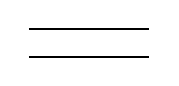
\begin{tikzpicture}[scale=0.45]
\draw[thick] (-1.7,0)--(1.7,0);
\draw[thick] (-1.7,0.8)--(1.7,0.8);
\end{tikzpicture}
\\
Zero curvature\\
Euclidean
};

\node (sph) [right=18mm of euc] {
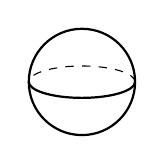
\begin{tikzpicture}[scale=0.45]
\draw[thick] (0,0) circle (1.5);
\draw[thick] (-1.5,0) arc (180:360:1.5 and 0.45);
\draw[dashed] (1.5,0) arc (0:180:1.5 and 0.45);
\end{tikzpicture}
\\
Positive curvature\\
Spherical
};

\end{tikzpicture}
\end{centereddiagram}

The drawings are schematic.

Curvature is an intrinsic mathematical quantity, not simply how a surface
appears when embedded in ordinary three-dimensional space.

%%%%%%%%%%%%%%%%%%%%%%%%%%%%%%%%%%%%%%%%%%%%%%%%%%%%%%%%%%%%
\subsection{Intrinsic Geometry}
\label{subsec:intrinsic-geometry}
%%%%%%%%%%%%%%%%%%%%%%%%%%%%%%%%%%%%%%%%%%%%%%%%%%%%%%%%%%%%

An inhabitant restricted to a surface could study distances and angles
without observing the surface from outside.

This motivates the idea of \emph{intrinsic geometry}.

\begin{definitionbox}{Intrinsic Geometry}
The \emph{intrinsic geometry} of a space consists of geometric properties
that can be determined entirely from measurements performed within the
space.
\end{definitionbox}

Distances, angles, geodesics, and curvature can be intrinsic quantities.

This idea becomes central in Differential Geometry and General Relativity.

%%%%%%%%%%%%%%%%%%%%%%%%%%%%%%%%%%%%%%%%%%%%%%%%%%%%%%%%%%%%
\subsection{Geodesics}
\label{subsec:non-euclidean-geodesics}
%%%%%%%%%%%%%%%%%%%%%%%%%%%%%%%%%%%%%%%%%%%%%%%%%%%%%%%%%%%%

In Euclidean geometry, straight lines represent shortest paths.

On curved spaces, the analogous objects are called \emph{geodesics}.

\begin{definitionbox}{Geodesic}
A \emph{geodesic} is a locally distance-minimizing path, or more generally a
curve satisfying the appropriate intrinsic straightness condition of the
geometry.
\end{definitionbox}

Examples include:

\[
\begin{array}{c|c}
\textbf{Geometry} & \textbf{Geodesics}\\
\hline
\text{Euclidean plane} & \text{straight lines}\\
\text{sphere} & \text{great circles}\\
\text{Poincar\'e disk} &
\text{special circular arcs or diameters}
\end{array}
\]

%%%%%%%%%%%%%%%%%%%%%%%%%%%%%%%%%%%%%%%%%%%%%%%%%%%%%%%%%%%%
\subsection{Hyperbolic Geometry}
\label{subsec:hyperbolic-geometry}
%%%%%%%%%%%%%%%%%%%%%%%%%%%%%%%%%%%%%%%%%%%%%%%%%%%%%%%%%%%%

Hyperbolic geometry is the classical geometry of constant negative
curvature.

Its parallel behavior differs dramatically from Euclidean geometry.

\begin{definitionbox}{Hyperbolic Parallel Property}
Given a hyperbolic line \(\ell\) and a point \(P\notin\ell\), infinitely
many hyperbolic lines through \(P\) do not intersect \(\ell\).
\end{definitionbox}

Thus

\[
\boxed{
\text{hyperbolic geometry has infinitely many parallels.}
}
\]

%%%%%%%%%%%%%%%%%%%%%%%%%%%%%%%%%%%%%%%%%%%%%%%%%%%%%%%%%%%%
\subsection{Why Models Are Useful}
\label{subsec:hyperbolic-models}
%%%%%%%%%%%%%%%%%%%%%%%%%%%%%%%%%%%%%%%%%%%%%%%%%%%%%%%%%%%%

Hyperbolic geometry cannot be represented globally inside the Euclidean
plane while preserving all Euclidean notions of distance and straightness.

Instead, mathematicians use \emph{models}.

A model represents hyperbolic points and lines using familiar Euclidean
objects while assigning them different geometric meanings.

Important models include:

\begin{itemize}
    \item the Poincar\'e disk model;
    \item the Poincar\'e upper half-plane model;
    \item the Klein disk model;
    \item the hyperboloid model.
\end{itemize}

These models describe the same underlying hyperbolic geometry in different
coordinates.

%%%%%%%%%%%%%%%%%%%%%%%%%%%%%%%%%%%%%%%%%%%%%%%%%%%%%%%%%%%%
\subsection{The Poincar\'e Disk Model}
\label{subsec:poincare-disk}
%%%%%%%%%%%%%%%%%%%%%%%%%%%%%%%%%%%%%%%%%%%%%%%%%%%%%%%%%%%%

The Poincar\'e disk model represents the hyperbolic plane inside the open
unit disk

\[
\boxed{
\mathbb{D}
=
\{(x,y)\in\R^2:x^2+y^2<1\}.
}
\]

The symbol

\[
\mathbb{D}
\]

is read ``the disk'' and here denotes the open unit disk.

The boundary circle

\[
x^2+y^2=1
\]

is not part of the hyperbolic plane.

%%%%%%%%%%%%%%%%%%%%%%%%%%%%%%%%%%%%%%%%%%%%%%%%%%%%%%%%%%%%
\subsection{Hyperbolic Lines in the Disk}
\label{subsec:hyperbolic-lines-disk}
%%%%%%%%%%%%%%%%%%%%%%%%%%%%%%%%%%%%%%%%%%%%%%%%%%%%%%%%%%%%

Hyperbolic lines in the Poincar\'e disk are represented by:

\begin{itemize}
    \item Euclidean diameters of the disk; or
    \item Euclidean circular arcs meeting the boundary circle
    orthogonally.
\end{itemize}

\begin{centereddiagram}
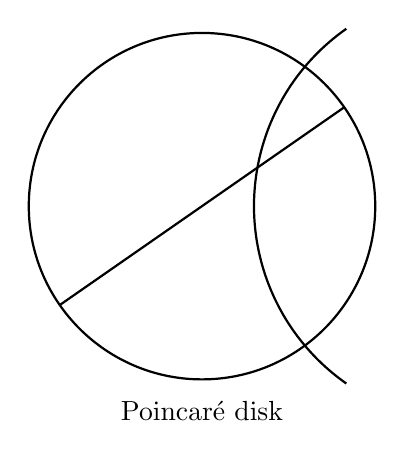
\begin{tikzpicture}[scale=2.2]
\draw[thick] (0,0) circle (1);

% diameter
\draw[thick] (-0.82,-0.57)--(0.82,0.57);

% orthogonal circular arc
\draw[thick,domain=125:235,samples=80]
plot ({1.55+1.25*cos(\x)},{1.25*sin(\x)});

\node at (0,-1.18) {Poincar\'e disk};
\end{tikzpicture}
\end{centereddiagram}

Although one of these ``lines'' appears curved in Euclidean coordinates, it
is straight from the hyperbolic viewpoint.

%%%%%%%%%%%%%%%%%%%%%%%%%%%%%%%%%%%%%%%%%%%%%%%%%%%%%%%%%%%%
\subsection{The Boundary at Infinity}
\label{subsec:hyperbolic-boundary-infinity}
%%%%%%%%%%%%%%%%%%%%%%%%%%%%%%%%%%%%%%%%%%%%%%%%%%%%%%%%%%%%

The boundary circle of the Poincar\'e disk is sometimes called the
\emph{ideal boundary} or \emph{boundary at infinity}.

Its points are not hyperbolic points.

Nevertheless, they represent asymptotic directions of hyperbolic geodesics.

A hyperbolic geodesic has two ideal endpoints on the boundary circle.

This resembles the use of ideal points in Projective Geometry, although the
structures are not identical.

%%%%%%%%%%%%%%%%%%%%%%%%%%%%%%%%%%%%%%%%%%%%%%%%%%%%%%%%%%%%
\subsection{Hyperbolic Parallels in the Disk}
\label{subsec:hyperbolic-parallels-disk}
%%%%%%%%%%%%%%%%%%%%%%%%%%%%%%%%%%%%%%%%%%%%%%%%%%%%%%%%%%%%

Let \(P\) be a point not on a hyperbolic line \(\ell\).

There are infinitely many hyperbolic lines through \(P\) that do not meet
\(\ell\) inside the disk.

\begin{centereddiagram}
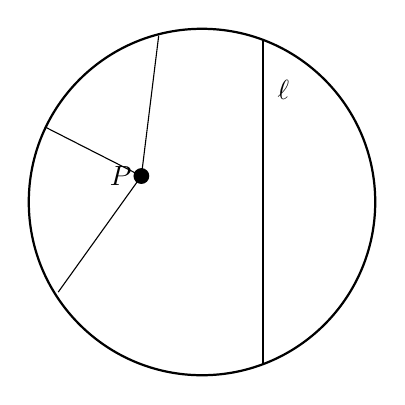
\begin{tikzpicture}[scale=2.2]
\draw[thick] (0,0) circle (1);

\coordinate (P) at (-0.35,0.15);
\fill (P) circle (1.3pt);
\node[left] at (P) {\(P\)};

% target line
\draw[thick] (0.35,-0.94)--(0.35,0.94);
\node[right] at (0.38,0.65) {\(\ell\)};

% schematic hyperbolic lines through P
\draw (-0.35,0.15)--(-0.90,0.43);
\draw (-0.35,0.15)--(-0.83,-0.52);
\draw (-0.35,0.15)--(-0.25,0.96);

\end{tikzpicture}
\end{centereddiagram}

The diagram is schematic; exact Poincar\'e geodesics must meet the boundary
orthogonally.

%%%%%%%%%%%%%%%%%%%%%%%%%%%%%%%%%%%%%%%%%%%%%%%%%%%%%%%%%%%%
\subsection{Conformal Geometry of the Poincar\'e Disk}
\label{subsec:poincare-conformal}
%%%%%%%%%%%%%%%%%%%%%%%%%%%%%%%%%%%%%%%%%%%%%%%%%%%%%%%%%%%%

One important property of the Poincar\'e disk model is that it is
\emph{conformal}.

\begin{definitionbox}{Conformal Model}
A geometric model is \emph{conformal} when it preserves angles between
intersecting curves.
\end{definitionbox}

Therefore Euclidean angles drawn inside the Poincar\'e disk equal the
corresponding hyperbolic angles.

Distances, however, are not Euclidean distances.

%%%%%%%%%%%%%%%%%%%%%%%%%%%%%%%%%%%%%%%%%%%%%%%%%%%%%%%%%%%%
\subsection{Hyperbolic Metric in the Disk}
\label{subsec:hyperbolic-metric-disk}
%%%%%%%%%%%%%%%%%%%%%%%%%%%%%%%%%%%%%%%%%%%%%%%%%%%%%%%%%%%%

For curvature normalized to

\[
K=-1,
\]

the Poincar\'e disk metric can be written

\[
\boxed{
ds^2
=
\frac{4(dx^2+dy^2)}
     {(1-x^2-y^2)^2}.
}
\]

The notation

\[
ds^2
\]

is read ``dee ess squared.''

It represents the infinitesimal squared distance determined by the metric.

As

\[
x^2+y^2\to1,
\]

the denominator approaches zero.

Thus the hyperbolic metric stretches dramatically near the boundary.

%%%%%%%%%%%%%%%%%%%%%%%%%%%%%%%%%%%%%%%%%%%%%%%%%%%%%%%%%%%%
\subsection{The Boundary Is Infinitely Far Away}
\label{subsec:hyperbolic-boundary-distance}
%%%%%%%%%%%%%%%%%%%%%%%%%%%%%%%%%%%%%%%%%%%%%%%%%%%%%%%%%%%%

Although the boundary circle appears at finite Euclidean distance, it lies at
infinite hyperbolic distance.

For example, along a radial path from the origin to radius \(r\),

\[
ds=\frac{2\,dr}{1-r^2}.
\]

Hence

\[
d(0,r)
=
\int_0^r\frac{2\,dt}{1-t^2}.
\]

Evaluating,

\[
\boxed{
d(0,r)
=
\ln\left(\frac{1+r}{1-r}\right).
}
\]

As

\[
r\to1^{-},
\]

we obtain

\[
d(0,r)\to\infty.
\]

%%%%%%%%%%%%%%%%%%%%%%%%%%%%%%%%%%%%%%%%%%%%%%%%%%%%%%%%%%%%
\subsection{Worked Example: Hyperbolic Radial Distance}
\label{subsec:worked-hyperbolic-radial-distance}
%%%%%%%%%%%%%%%%%%%%%%%%%%%%%%%%%%%%%%%%%%%%%%%%%%%%%%%%%%%%

\begin{workedexamplebox}{Distance from the Origin}

Find the hyperbolic distance from the origin to a point whose Euclidean
radius is

\[
r=\frac12
\]

in the curvature-\(-1\) Poincar\'e disk.

Use

\[
d(0,r)
=
\ln\left(\frac{1+r}{1-r}\right).
\]

Then

\[
d\left(0,\frac12\right)
=
\ln
\left(
\frac{1+\frac12}{1-\frac12}
\right).
\]

Therefore

\[
=
\ln\left(\frac{3/2}{1/2}\right)
=
\ln3.
\]

\begin{answerbox}
\[
\boxed{
d\left(0,\frac12\right)=\ln3
}
\]
\end{answerbox}
\end{workedexamplebox}

%%%%%%%%%%%%%%%%%%%%%%%%%%%%%%%%%%%%%%%%%%%%%%%%%%%%%%%%%%%%
\subsection{Distance Between Two Disk Points}
\label{subsec:hyperbolic-distance-disk}
%%%%%%%%%%%%%%%%%%%%%%%%%%%%%%%%%%%%%%%%%%%%%%%%%%%%%%%%%%%%

For points

\[
u,v\in\mathbb{D},
\]

one useful distance formula is

\[
\boxed{
\cosh d(u,v)
=
1+
\frac{2\|u-v\|^2}
{(1-\|u\|^2)(1-\|v\|^2)}.
}
\]

Here

\[
\cosh
\]

denotes the hyperbolic cosine.

It is defined by

\[
\boxed{
\cosh t=\frac{e^t+e^{-t}}{2}.
}
\]

The Euclidean norm \(\|\cdot\|\) appears in the coordinate formula, but the
resulting distance is hyperbolic.

%%%%%%%%%%%%%%%%%%%%%%%%%%%%%%%%%%%%%%%%%%%%%%%%%%%%%%%%%%%%
\subsection{The Poincar\'e Upper Half-Plane}
\label{subsec:poincare-upper-half-plane}
%%%%%%%%%%%%%%%%%%%%%%%%%%%%%%%%%%%%%%%%%%%%%%%%%%%%%%%%%%%%

Another important model is the upper half-plane

\[
\boxed{
\mathbb{H}
=
\{(x,y)\in\R^2:y>0\}.
}
\]

The symbol

\[
\mathbb{H}
\]

is read ``the upper half-plane'' in this context.

Its boundary is the real axis together with an ideal point at infinity.

%%%%%%%%%%%%%%%%%%%%%%%%%%%%%%%%%%%%%%%%%%%%%%%%%%%%%%%%%%%%
\subsection{Lines in the Upper Half-Plane}
\label{subsec:upper-half-plane-lines}
%%%%%%%%%%%%%%%%%%%%%%%%%%%%%%%%%%%%%%%%%%%%%%%%%%%%%%%%%%%%

Hyperbolic lines in the upper half-plane model are:

\begin{itemize}
    \item vertical Euclidean lines; or
    \item semicircles orthogonal to the real axis.
\end{itemize}

\begin{centereddiagram}
\begin{tikzpicture}[scale=0.9]
\draw[->] (-4,0)--(4,0) node[right] {\(x\)};
\draw[->] (0,0)--(0,4) node[above] {\(y\)};

\draw[thick] (-2,0)--(-2,3.5);

\draw[thick,domain=0:180,samples=80]
plot ({1.2+1.5*cos(\x)},{1.5*sin(\x)});

\node at (2.8,3.4) {\(\mathbb{H}\)};
\end{tikzpicture}
\end{centereddiagram}

Like the disk model, the upper half-plane model is conformal.

%%%%%%%%%%%%%%%%%%%%%%%%%%%%%%%%%%%%%%%%%%%%%%%%%%%%%%%%%%%%
\subsection{Upper Half-Plane Metric}
\label{subsec:upper-half-plane-metric}
%%%%%%%%%%%%%%%%%%%%%%%%%%%%%%%%%%%%%%%%%%%%%%%%%%%%%%%%%%%%

For curvature

\[
K=-1,
\]

the hyperbolic metric on the upper half-plane is

\[
\boxed{
ds^2
=
\frac{dx^2+dy^2}{y^2}.
}
\]

As

\[
y\to0^{+},
\]

the metric stretches.

Therefore the real axis is infinitely far away in hyperbolic distance.

%%%%%%%%%%%%%%%%%%%%%%%%%%%%%%%%%%%%%%%%%%%%%%%%%%%%%%%%%%%%
\subsection{Vertical Hyperbolic Distance}
\label{subsec:vertical-hyperbolic-distance}
%%%%%%%%%%%%%%%%%%%%%%%%%%%%%%%%%%%%%%%%%%%%%%%%%%%%%%%%%%%%

Consider two points on a vertical geodesic:

\[
P=(x,y_1),
\qquad
Q=(x,y_2).
\]

Since

\[
dx=0,
\]

the metric gives

\[
ds=\frac{|dy|}{y}.
\]

Therefore

\[
d(P,Q)
=
\left|
\int_{y_1}^{y_2}\frac{dy}{y}
\right|.
\]

Hence

\[
\boxed{
d(P,Q)
=
\left|
\ln\frac{y_2}{y_1}
\right|.
}
\]

%%%%%%%%%%%%%%%%%%%%%%%%%%%%%%%%%%%%%%%%%%%%%%%%%%%%%%%%%%%%
\subsection{Worked Example: Upper Half-Plane Distance}
\label{subsec:worked-upper-half-plane-distance}
%%%%%%%%%%%%%%%%%%%%%%%%%%%%%%%%%%%%%%%%%%%%%%%%%%%%%%%%%%%%

\begin{workedexamplebox}{Vertical Hyperbolic Distance}

Find the hyperbolic distance between

\[
P=(2,1)
\]

and

\[
Q=(2,4).
\]

Since the points lie on the same vertical geodesic,

\[
d(P,Q)
=
\left|
\ln\frac{4}{1}
\right|.
\]

Therefore

\[
\boxed{d(P,Q)=\ln4.}
\]

\begin{answerbox}
\[
\boxed{d(P,Q)=\ln4}
\]
\end{answerbox}
\end{workedexamplebox}

%%%%%%%%%%%%%%%%%%%%%%%%%%%%%%%%%%%%%%%%%%%%%%%%%%%%%%%%%%%%
\subsection{Disk and Half-Plane Models}
\label{subsec:disk-half-plane-equivalence}
%%%%%%%%%%%%%%%%%%%%%%%%%%%%%%%%%%%%%%%%%%%%%%%%%%%%%%%%%%%%

The Poincar\'e disk and upper half-plane are not different hyperbolic
geometries.

They are different models of the same geometry.

In complex notation, one transformation from the upper half-plane to the
unit disk is

\[
\boxed{
w=\frac{z-i}{z+i}.
}
\]

Here

\[
z=x+iy
\]

is a complex coordinate.

This fractional linear transformation maps

\[
\mathbb{H}
\]

onto

\[
\mathbb{D}.
\]

The relationship is studied further in Complex Analysis.

%%%%%%%%%%%%%%%%%%%%%%%%%%%%%%%%%%%%%%%%%%%%%%%%%%%%%%%%%%%%
\subsection{The Klein Disk Model}
\label{subsec:klein-disk}
%%%%%%%%%%%%%%%%%%%%%%%%%%%%%%%%%%%%%%%%%%%%%%%%%%%%%%%%%%%%

The Klein disk model also represents the hyperbolic plane inside a disk.

Its geodesics are Euclidean chords of the disk.

This makes incidence particularly simple.

However, unlike the Poincar\'e disk, the Klein model is not conformal.

Thus Euclidean angles in the picture are generally not hyperbolic angles.

\[
\boxed{
\begin{array}{c|c|c}
& \textbf{Geodesics} & \textbf{Conformal}\\
\hline
\text{Poincar\'e disk} &
\text{orthogonal arcs} &
\text{yes}\\
\text{Klein disk} &
\text{chords} &
\text{no}
\end{array}
}
\]

%%%%%%%%%%%%%%%%%%%%%%%%%%%%%%%%%%%%%%%%%%%%%%%%%%%%%%%%%%%%
\subsection{The Hyperboloid Model}
\label{subsec:hyperboloid-model}
%%%%%%%%%%%%%%%%%%%%%%%%%%%%%%%%%%%%%%%%%%%%%%%%%%%%%%%%%%%%

Hyperbolic geometry can also be represented using a surface in
three-dimensional Minkowski space.

One common model uses

\[
\boxed{
-x_0^2+x_1^2+x_2^2=-1,
\qquad
x_0>0.
}
\]

This is one sheet of a two-sheeted hyperboloid.

The ambient bilinear form is not the ordinary Euclidean dot product.

Instead, one uses a Lorentzian form such as

\[
\boxed{
\langle x,y\rangle_L
=
-x_0y_0+x_1y_1+x_2y_2.
}
\]

The subscript \(L\) indicates ``Lorentzian.''

This model creates an important connection between hyperbolic geometry and
special relativity.

%%%%%%%%%%%%%%%%%%%%%%%%%%%%%%%%%%%%%%%%%%%%%%%%%%%%%%%%%%%%
\subsection{Hyperbolic Triangle Angle Sum}
\label{subsec:hyperbolic-triangle-angle-sum}
%%%%%%%%%%%%%%%%%%%%%%%%%%%%%%%%%%%%%%%%%%%%%%%%%%%%%%%%%%%%

One of the most striking differences from Euclidean geometry concerns
triangles.

In Euclidean geometry,

\[
\alpha+\beta+\gamma=\pi.
\]

In hyperbolic geometry,

\[
\boxed{
\alpha+\beta+\gamma<\pi.
}
\]

The quantity

\[
\boxed{
\delta
=
\pi-(\alpha+\beta+\gamma)
}
\]

is called the \emph{angle defect} of the hyperbolic triangle.

The Greek letter

\[
\delta
\]

is read ``delta.''

%%%%%%%%%%%%%%%%%%%%%%%%%%%%%%%%%%%%%%%%%%%%%%%%%%%%%%%%%%%%
\subsection{Hyperbolic Triangle Area}
\label{subsec:hyperbolic-triangle-area}
%%%%%%%%%%%%%%%%%%%%%%%%%%%%%%%%%%%%%%%%%%%%%%%%%%%%%%%%%%%%

For a hyperbolic plane of constant curvature

\[
K=-1,
\]

the area of a geodesic triangle is

\[
\boxed{
A
=
\pi-(\alpha+\beta+\gamma).
}
\]

Thus

\[
\boxed{
A=\delta.
}
\]

More generally, if the curvature is

\[
K=-\frac{1}{R^2},
\]

then

\[
\boxed{
A
=
R^2
\left[
\pi-(\alpha+\beta+\gamma)
\right].
}
\]

This is a profound contrast with Euclidean geometry: the angles determine the
area.

%%%%%%%%%%%%%%%%%%%%%%%%%%%%%%%%%%%%%%%%%%%%%%%%%%%%%%%%%%%%
\subsection{Worked Example: Hyperbolic Triangle Area}
\label{subsec:worked-hyperbolic-triangle-area}
%%%%%%%%%%%%%%%%%%%%%%%%%%%%%%%%%%%%%%%%%%%%%%%%%%%%%%%%%%%%

\begin{workedexamplebox}{Area from Hyperbolic Angles}

Suppose a hyperbolic triangle in curvature \(K=-1\) has angles

\[
\alpha=\frac{\pi}{3},
\qquad
\beta=\frac{\pi}{4},
\qquad
\gamma=\frac{\pi}{6}.
\]

Its angle sum is

\[
\frac{\pi}{3}
+
\frac{\pi}{4}
+
\frac{\pi}{6}.
\]

Using denominator \(12\),

\[
=
\frac{4\pi+3\pi+2\pi}{12}
=
\frac{9\pi}{12}
=
\frac{3\pi}{4}.
\]

Therefore

\[
A
=
\pi-\frac{3\pi}{4}
=
\frac{\pi}{4}.
\]

\begin{answerbox}
\[
\boxed{A=\frac{\pi}{4}}
\]
\end{answerbox}
\end{workedexamplebox}

%%%%%%%%%%%%%%%%%%%%%%%%%%%%%%%%%%%%%%%%%%%%%%%%%%%%%%%%%%%%
\subsection{Ideal Triangles}
\label{subsec:ideal-hyperbolic-triangles}
%%%%%%%%%%%%%%%%%%%%%%%%%%%%%%%%%%%%%%%%%%%%%%%%%%%%%%%%%%%%

A hyperbolic triangle whose vertices lie on the ideal boundary is called an
\emph{ideal triangle}.

Its interior angles are all zero:

\[
\alpha=\beta=\gamma=0.
\]

Therefore, in curvature \(K=-1\),

\[
\boxed{
A=\pi.
}
\]

Thus an ideal triangle has finite area even though its vertices are
infinitely far away.

%%%%%%%%%%%%%%%%%%%%%%%%%%%%%%%%%%%%%%%%%%%%%%%%%%%%%%%%%%%%
\subsection{Hyperbolic Polygons}
\label{subsec:hyperbolic-polygons}
%%%%%%%%%%%%%%%%%%%%%%%%%%%%%%%%%%%%%%%%%%%%%%%%%%%%%%%%%%%%

For a geodesic \(n\)-gon in curvature \(K=-1\), with interior angles

\[
\alpha_1,\ldots,\alpha_n,
\]

the area is

\[
\boxed{
A
=
(n-2)\pi
-
\sum_{k=1}^{n}\alpha_k.
}
\]

The Euclidean angle-sum formula

\[
(n-2)\pi
\]

therefore becomes an upper bound for the angle sum of a hyperbolic polygon.

%%%%%%%%%%%%%%%%%%%%%%%%%%%%%%%%%%%%%%%%%%%%%%%%%%%%%%%%%%%%
\subsection{Hyperbolic Circles}
\label{subsec:hyperbolic-circles}
%%%%%%%%%%%%%%%%%%%%%%%%%%%%%%%%%%%%%%%%%%%%%%%%%%%%%%%%%%%%

Hyperbolic circles grow more rapidly than Euclidean circles.

For curvature \(K=-1\), a hyperbolic circle of radius \(r\) has circumference

\[
\boxed{
C(r)=2\pi\sinh r
}
\]

and area

\[
\boxed{
A(r)=2\pi(\cosh r-1).
}
\]

The hyperbolic sine is

\[
\boxed{
\sinh r=\frac{e^r-e^{-r}}{2}.
}
\]

For large \(r\),

\[
\sinh r
\]

and

\[
\cosh r
\]

grow exponentially.

This reflects the rapid expansion of negatively curved space.

%%%%%%%%%%%%%%%%%%%%%%%%%%%%%%%%%%%%%%%%%%%%%%%%%%%%%%%%%%%%
\subsection{Comparison with Euclidean Circle Growth}
\label{subsec:circle-growth-comparison}
%%%%%%%%%%%%%%%%%%%%%%%%%%%%%%%%%%%%%%%%%%%%%%%%%%%%%%%%%%%%

In Euclidean geometry,

\[
C_E(r)=2\pi r
\]

and

\[
A_E(r)=\pi r^2.
\]

In hyperbolic geometry,

\[
C_H(r)=2\pi\sinh r
\]

and

\[
A_H(r)=2\pi(\cosh r-1).
\]

Near

\[
r=0,
\]

the hyperbolic formulas resemble the Euclidean formulas.

For large \(r\), they diverge dramatically.

This demonstrates how Euclidean geometry can appear locally accurate even
when the global geometry is non-Euclidean.

%%%%%%%%%%%%%%%%%%%%%%%%%%%%%%%%%%%%%%%%%%%%%%%%%%%%%%%%%%%%
\subsection{Hyperbolic Trigonometry}
\label{subsec:hyperbolic-trigonometry}
%%%%%%%%%%%%%%%%%%%%%%%%%%%%%%%%%%%%%%%%%%%%%%%%%%%%%%%%%%%%

Triangle formulas also change.

For a hyperbolic triangle with side lengths

\[
a,b,c
\]

opposite angles

\[
A,B,C,
\]

the hyperbolic law of cosines for curvature \(K=-1\) is

\[
\boxed{
\cosh c
=
\cosh a\cosh b
-
\sinh a\sinh b\cos C.
}
\]

Compare this with the Euclidean law of cosines:

\[
c^2=a^2+b^2-2ab\cos C.
\]

%%%%%%%%%%%%%%%%%%%%%%%%%%%%%%%%%%%%%%%%%%%%%%%%%%%%%%%%%%%%
\subsection{Hyperbolic Law of Sines}
\label{subsec:hyperbolic-law-sines}
%%%%%%%%%%%%%%%%%%%%%%%%%%%%%%%%%%%%%%%%%%%%%%%%%%%%%%%%%%%%

The hyperbolic law of sines is

\[
\boxed{
\frac{\sin A}{\sinh a}
=
\frac{\sin B}{\sinh b}
=
\frac{\sin C}{\sinh c}.
}
\]

Ordinary trigonometric functions appear for angles, while hyperbolic
functions appear naturally for side lengths.

%%%%%%%%%%%%%%%%%%%%%%%%%%%%%%%%%%%%%%%%%%%%%%%%%%%%%%%%%%%%
\subsection{Right Hyperbolic Triangles}
\label{subsec:right-hyperbolic-triangles}
%%%%%%%%%%%%%%%%%%%%%%%%%%%%%%%%%%%%%%%%%%%%%%%%%%%%%%%%%%%%

If

\[
C=\frac{\pi}{2},
\]

then

\[
\cos C=0.
\]

The hyperbolic law of cosines becomes

\[
\boxed{
\cosh c
=
\cosh a\cosh b.
}
\]

This is the hyperbolic analogue of the Pythagorean theorem.

For very small side lengths, it approximates

\[
c^2\approx a^2+b^2.
\]

%%%%%%%%%%%%%%%%%%%%%%%%%%%%%%%%%%%%%%%%%%%%%%%%%%%%%%%%%%%%
\subsection{Local Euclidean Approximation}
\label{subsec:local-euclidean-approximation}
%%%%%%%%%%%%%%%%%%%%%%%%%%%%%%%%%%%%%%%%%%%%%%%%%%%%%%%%%%%%

For small \(t\),

\[
\sinh t
=
t+O(t^3)
\]

and

\[
\cosh t
=
1+\frac{t^2}{2}+O(t^4).
\]

Substituting these approximations into hyperbolic formulas recovers
Euclidean formulas to leading order.

Thus:

\[
\boxed{
\text{small regions of a smooth curved geometry look approximately
Euclidean.}
}
\]

This principle is fundamental in differential geometry.

%%%%%%%%%%%%%%%%%%%%%%%%%%%%%%%%%%%%%%%%%%%%%%%%%%%%%%%%%%%%
\subsection{Spherical Geometry}
\label{subsec:spherical-geometry}
%%%%%%%%%%%%%%%%%%%%%%%%%%%%%%%%%%%%%%%%%%%%%%%%%%%%%%%%%%%%

Positive-curvature geometry can be modeled using a sphere.

Consider the sphere of radius \(R\):

\[
\boxed{
x^2+y^2+z^2=R^2.
}
\]

Its intrinsic geometry is called \emph{spherical geometry}.

The natural analogues of straight lines are great circles.

%%%%%%%%%%%%%%%%%%%%%%%%%%%%%%%%%%%%%%%%%%%%%%%%%%%%%%%%%%%%
\subsection{Great Circles}
\label{subsec:great-circles}
%%%%%%%%%%%%%%%%%%%%%%%%%%%%%%%%%%%%%%%%%%%%%%%%%%%%%%%%%%%%

\begin{definitionbox}{Great Circle}
A \emph{great circle} on a sphere is the intersection of the sphere with a
plane passing through the center of the sphere.
\end{definitionbox}

Examples on Earth include:

\begin{itemize}
    \item the equator;
    \item any complete meridian together with its opposite meridian.
\end{itemize}

Great circles are geodesics of the sphere.

%%%%%%%%%%%%%%%%%%%%%%%%%%%%%%%%%%%%%%%%%%%%%%%%%%%%%%%%%%%%
\subsection{Great-Circle Distance}
\label{subsec:great-circle-distance}
%%%%%%%%%%%%%%%%%%%%%%%%%%%%%%%%%%%%%%%%%%%%%%%%%%%%%%%%%%%%

Suppose two points on a sphere of radius \(R\) subtend a central angle

\[
\theta.
\]

The geodesic distance along the shorter great-circle arc is

\[
\boxed{
d=R\theta.
}
\]

Here \(\theta\) must be measured in radians.

This formula is widely used in navigation and geodesy.

%%%%%%%%%%%%%%%%%%%%%%%%%%%%%%%%%%%%%%%%%%%%%%%%%%%%%%%%%%%%
\subsection{Distance from Dot Products}
\label{subsec:spherical-distance-dot-product}
%%%%%%%%%%%%%%%%%%%%%%%%%%%%%%%%%%%%%%%%%%%%%%%%%%%%%%%%%%%%

Let

\[
\mathbf{u},\mathbf{v}\in\R^3
\]

represent points on a sphere of radius \(R\).

Then

\[
\mathbf{u}\cdot\mathbf{v}
=
R^2\cos\theta.
\]

Therefore

\[
\boxed{
\theta
=
\arccos
\left(
\frac{\mathbf{u}\cdot\mathbf{v}}{R^2}
\right).
}
\]

Hence

\[
\boxed{
d
=
R\arccos
\left(
\frac{\mathbf{u}\cdot\mathbf{v}}{R^2}
\right).
}
\]

%%%%%%%%%%%%%%%%%%%%%%%%%%%%%%%%%%%%%%%%%%%%%%%%%%%%%%%%%%%%
\subsection{Worked Example: Great-Circle Distance}
\label{subsec:worked-great-circle-distance}
%%%%%%%%%%%%%%%%%%%%%%%%%%%%%%%%%%%%%%%%%%%%%%%%%%%%%%%%%%%%

\begin{workedexamplebox}{Distance on the Unit Sphere}

Let

\[
P=(1,0,0)
\]

and

\[
Q=(0,1,0)
\]

lie on the unit sphere.

Compute

\[
P\cdot Q=0.
\]

Thus

\[
\cos\theta=0,
\]

so

\[
\theta=\frac{\pi}{2}.
\]

Since

\[
R=1,
\]

the spherical distance is

\[
d=R\theta=\frac{\pi}{2}.
\]

\begin{answerbox}
\[
\boxed{d=\frac{\pi}{2}}
\]
\end{answerbox}
\end{workedexamplebox}

%%%%%%%%%%%%%%%%%%%%%%%%%%%%%%%%%%%%%%%%%%%%%%%%%%%%%%%%%%%%
\subsection{No Parallel Great Circles}
\label{subsec:no-parallel-great-circles}
%%%%%%%%%%%%%%%%%%%%%%%%%%%%%%%%%%%%%%%%%%%%%%%%%%%%%%%%%%%%

Any two distinct great circles on a sphere intersect in two antipodal
points.

Therefore spherical geometry has no ordinary parallel geodesics.

This gives the positive-curvature analogue of the parallel postulate:

\[
\boxed{
\text{through a point outside a geodesic, there are no parallel geodesics.}
}
\]

There is one subtlety: two great circles intersect twice rather than once.

Elliptic geometry removes this duplication by identifying antipodal points.

%%%%%%%%%%%%%%%%%%%%%%%%%%%%%%%%%%%%%%%%%%%%%%%%%%%%%%%%%%%%
\subsection{Elliptic Geometry}
\label{subsec:elliptic-geometry}
%%%%%%%%%%%%%%%%%%%%%%%%%%%%%%%%%%%%%%%%%%%%%%%%%%%%%%%%%%%%

\begin{definitionbox}{Elliptic Geometry}
\emph{Elliptic geometry} can be modeled by spherical geometry with antipodal
points identified:

\[
\boxed{
\mathbf{x}\sim-\mathbf{x}.
}
\]
\end{definitionbox}

Thus opposite points on the sphere represent the same elliptic point.

Under this identification, two distinct elliptic lines intersect exactly
once.

The elliptic plane is closely related to the real projective plane

\[
\mathbb{P}^{2}(\R).
\]

%%%%%%%%%%%%%%%%%%%%%%%%%%%%%%%%%%%%%%%%%%%%%%%%%%%%%%%%%%%%
\subsection{Spherical Triangle Angle Sum}
\label{subsec:spherical-triangle-angle-sum}
%%%%%%%%%%%%%%%%%%%%%%%%%%%%%%%%%%%%%%%%%%%%%%%%%%%%%%%%%%%%

A spherical triangle is formed by three great-circle arcs.

Unlike Euclidean triangles,

\[
\boxed{
\alpha+\beta+\gamma>\pi.
}
\]

The quantity

\[
\boxed{
E
=
\alpha+\beta+\gamma-\pi
}
\]

is called the \emph{spherical excess}.

%%%%%%%%%%%%%%%%%%%%%%%%%%%%%%%%%%%%%%%%%%%%%%%%%%%%%%%%%%%%
\subsection{Area of a Spherical Triangle}
\label{subsec:spherical-triangle-area}
%%%%%%%%%%%%%%%%%%%%%%%%%%%%%%%%%%%%%%%%%%%%%%%%%%%%%%%%%%%%

For a sphere of radius \(R\), the area of a spherical triangle is

\[
\boxed{
A
=
R^2
(\alpha+\beta+\gamma-\pi).
}
\]

Thus

\[
\boxed{
A=R^2E.
}
\]

For the unit sphere,

\[
R=1,
\]

so

\[
\boxed{
A=\alpha+\beta+\gamma-\pi.
}
\]

Again, triangle angles determine area.

%%%%%%%%%%%%%%%%%%%%%%%%%%%%%%%%%%%%%%%%%%%%%%%%%%%%%%%%%%%%
\subsection{Worked Example: Spherical Triangle}
\label{subsec:worked-spherical-triangle}
%%%%%%%%%%%%%%%%%%%%%%%%%%%%%%%%%%%%%%%%%%%%%%%%%%%%%%%%%%%%

\begin{workedexamplebox}{A Triangle with Three Right Angles}

Consider a spherical triangle on the unit sphere with

\[
\alpha=\beta=\gamma=\frac{\pi}{2}.
\]

Its angle sum is

\[
\frac{3\pi}{2}.
\]

The spherical excess is

\[
E
=
\frac{3\pi}{2}-\pi
=
\frac{\pi}{2}.
\]

Since \(R=1\),

\[
A=E.
\]

\begin{answerbox}
\[
\boxed{A=\frac{\pi}{2}}
\]
\end{answerbox}

Such a triangle is impossible in Euclidean geometry but perfectly natural on
a sphere.
\end{workedexamplebox}

%%%%%%%%%%%%%%%%%%%%%%%%%%%%%%%%%%%%%%%%%%%%%%%%%%%%%%%%%%%%
\subsection{A Concrete Three-Right-Angle Triangle}
\label{subsec:three-right-angle-triangle}
%%%%%%%%%%%%%%%%%%%%%%%%%%%%%%%%%%%%%%%%%%%%%%%%%%%%%%%%%%%%

Take:

\begin{itemize}
    \item the North Pole;
    \item one point on the equator;
    \item another equatorial point \(90^\circ\) away.
\end{itemize}

Connect them using two meridians and the equator.

Each interior angle equals

\[
90^\circ.
\]

Thus

\[
\boxed{
90^\circ+90^\circ+90^\circ=270^\circ.
}
\]

This is one of the simplest demonstrations that Euclidean triangle geometry
does not apply globally on a sphere.

%%%%%%%%%%%%%%%%%%%%%%%%%%%%%%%%%%%%%%%%%%%%%%%%%%%%%%%%%%%%
\subsection{Spherical Law of Cosines}
\label{subsec:spherical-law-cosines}
%%%%%%%%%%%%%%%%%%%%%%%%%%%%%%%%%%%%%%%%%%%%%%%%%%%%%%%%%%%%

On a unit sphere, let a spherical triangle have side lengths

\[
a,b,c
\]

measured as central angles, with opposite angles

\[
A,B,C.
\]

Then

\[
\boxed{
\cos c
=
\cos a\cos b
+
\sin a\sin b\cos C.
}
\]

For a sphere of radius \(R\), one may replace the angular side lengths by

\[
\frac{a}{R},
\qquad
\frac{b}{R},
\qquad
\frac{c}{R}.
\]

%%%%%%%%%%%%%%%%%%%%%%%%%%%%%%%%%%%%%%%%%%%%%%%%%%%%%%%%%%%%
\subsection{Spherical Law of Sines}
\label{subsec:spherical-law-sines}
%%%%%%%%%%%%%%%%%%%%%%%%%%%%%%%%%%%%%%%%%%%%%%%%%%%%%%%%%%%%

The spherical law of sines is

\[
\boxed{
\frac{\sin A}{\sin a}
=
\frac{\sin B}{\sin b}
=
\frac{\sin C}{\sin c}
}
\]

when side lengths are measured as central angles on the unit sphere.

These formulas are essential in spherical astronomy, geodesy, and
navigation.

%%%%%%%%%%%%%%%%%%%%%%%%%%%%%%%%%%%%%%%%%%%%%%%%%%%%%%%%%%%%
\subsection{Comparison of Triangle Angle Sums}
\label{subsec:triangle-angle-sum-comparison}
%%%%%%%%%%%%%%%%%%%%%%%%%%%%%%%%%%%%%%%%%%%%%%%%%%%%%%%%%%%%

Triangle angle sums provide a direct signature of curvature.

\[
\boxed{
\begin{array}{c|c}
\textbf{Geometry} & \textbf{Triangle angle sum}\\
\hline
\text{Hyperbolic} &
\alpha+\beta+\gamma<\pi\\
\text{Euclidean} &
\alpha+\beta+\gamma=\pi\\
\text{Spherical / Elliptic} &
\alpha+\beta+\gamma>\pi
\end{array}
}
\]

This pattern reflects negative, zero, and positive curvature.

%%%%%%%%%%%%%%%%%%%%%%%%%%%%%%%%%%%%%%%%%%%%%%%%%%%%%%%%%%%%
\subsection{Area and Angle Defect}
\label{subsec:area-angle-defect}
%%%%%%%%%%%%%%%%%%%%%%%%%%%%%%%%%%%%%%%%%%%%%%%%%%%%%%%%%%%%

For constant curvature, triangle area is directly related to the departure
of the angle sum from \(\pi\).

For curvature \(K\neq0\),

\[
\boxed{
K A
=
\alpha+\beta+\gamma-\pi.
}
\]

For \(K>0\), the right-hand side is positive.

For \(K<0\), it is negative.

Solving for area gives the appropriate positive value in each case.

This formula is a special case of the deeper Gauss--Bonnet theorem.

%%%%%%%%%%%%%%%%%%%%%%%%%%%%%%%%%%%%%%%%%%%%%%%%%%%%%%%%%%%%
\subsection{Gauss--Bonnet Preview}
\label{subsec:gauss-bonnet-preview}
%%%%%%%%%%%%%%%%%%%%%%%%%%%%%%%%%%%%%%%%%%%%%%%%%%%%%%%%%%%%

The relationship between curvature, angles, area, and topology is generalized
by one of the central results of differential geometry.

For a suitable compact surface \(S\),

\[
\boxed{
\int_S K\,dA
=
2\pi\chi(S).
}
\]

The symbol

\[
\chi
\]

is the Greek letter chi, pronounced ``kai'' in common mathematical English.

Here

\[
\chi(S)
\]

denotes the Euler characteristic of the surface.

The full Gauss--Bonnet theorem is developed later in Differential Geometry.

%%%%%%%%%%%%%%%%%%%%%%%%%%%%%%%%%%%%%%%%%%%%%%%%%%%%%%%%%%%%
\subsection{Saccheri Quadrilaterals}
\label{subsec:saccheri-quadrilaterals}
%%%%%%%%%%%%%%%%%%%%%%%%%%%%%%%%%%%%%%%%%%%%%%%%%%%%%%%%%%%%

Historically, attempts to prove the parallel postulate often used special
quadrilaterals.

\begin{definitionbox}{Saccheri Quadrilateral}
A \emph{Saccheri quadrilateral} is a quadrilateral \(ABCD\) satisfying

\[
AD=BC
\]

and

\[
\angle A=\angle B=\frac{\pi}{2},
\]

where \(AB\) is the base and \(CD\) is the summit.
\end{definitionbox}

The summit angles reveal the geometry:

\[
\begin{array}{c|c}
\textbf{Geometry} & \textbf{Summit angles}\\
\hline
\text{Hyperbolic} & <\frac{\pi}{2}\\
\text{Euclidean} & =\frac{\pi}{2}\\
\text{Elliptic-type behavior} & >\frac{\pi}{2}
\end{array}
\]

Historically, studying these possibilities helped reveal that alternative
geometries could be logically consistent.

%%%%%%%%%%%%%%%%%%%%%%%%%%%%%%%%%%%%%%%%%%%%%%%%%%%%%%%%%%%%
\subsection{The Angle of Parallelism}
\label{subsec:angle-of-parallelism}
%%%%%%%%%%%%%%%%%%%%%%%%%%%%%%%%%%%%%%%%%%%%%%%%%%%%%%%%%%%%

Hyperbolic geometry has a quantity with no Euclidean analogue.

Suppose \(P\) lies a perpendicular distance \(d\) from a line.

The limiting parallel geodesics make an angle

\[
\Pi(d)
\]

with the perpendicular.

The Greek capital letter

\[
\Pi
\]

is read ``capital pi.''

For curvature \(K=-1\),

\[
\boxed{
\tan\left(\frac{\Pi(d)}{2}\right)=e^{-d}.
}
\]

Equivalently,

\[
\boxed{
\Pi(d)
=
2\arctan(e^{-d}).
}
\]

As

\[
d\to0,
\]

we have

\[
\Pi(d)\to\frac{\pi}{2}.
\]

As

\[
d\to\infty,
\]

we have

\[
\Pi(d)\to0.
\]

%%%%%%%%%%%%%%%%%%%%%%%%%%%%%%%%%%%%%%%%%%%%%%%%%%%%%%%%%%%%
\subsection{Absolute Geometry}
\label{subsec:absolute-geometry}
%%%%%%%%%%%%%%%%%%%%%%%%%%%%%%%%%%%%%%%%%%%%%%%%%%%%%%%%%%%%

Many results of Euclidean geometry do not require the parallel postulate.

The geometry obtained from the common axioms before choosing a parallel
postulate is often called \emph{absolute geometry} or \emph{neutral
geometry}.

This distinction helps separate:

\[
\boxed{
\text{results depending on parallelism}
}
\]

from

\[
\boxed{
\text{results valid more generally}.
}
\]

%%%%%%%%%%%%%%%%%%%%%%%%%%%%%%%%%%%%%%%%%%%%%%%%%%%%%%%%%%%%
\subsection{Consistency of Non-Euclidean Geometry}
\label{subsec:consistency-non-euclidean}
%%%%%%%%%%%%%%%%%%%%%%%%%%%%%%%%%%%%%%%%%%%%%%%%%%%%%%%%%%%%

The discovery of concrete models had a major logical consequence.

If a model of hyperbolic geometry can be constructed using ordinary
Euclidean mathematics, then a contradiction in hyperbolic geometry would
produce a contradiction in the Euclidean framework used to construct the
model.

Thus models provide \emph{relative consistency} results.

They showed that the parallel postulate cannot simply be derived from the
remaining Euclidean axioms, assuming the consistency of the background
system.

%%%%%%%%%%%%%%%%%%%%%%%%%%%%%%%%%%%%%%%%%%%%%%%%%%%%%%%%%%%%
\subsection{Historical Development}
\label{subsec:non-euclidean-history}
%%%%%%%%%%%%%%%%%%%%%%%%%%%%%%%%%%%%%%%%%%%%%%%%%%%%%%%%%%%%

For roughly two thousand years, mathematicians attempted to prove Euclid's
parallel postulate from the other axioms.

Important contributors to the eventual development of non-Euclidean geometry
include:

\begin{itemize}
    \item Giovanni Girolamo Saccheri;
    \item Johann Heinrich Lambert;
    \item Carl Friedrich Gauss;
    \item Nikolai Lobachevsky;
    \item J\'anos Bolyai;
    \item Bernhard Riemann;
    \item Eugenio Beltrami;
    \item Felix Klein;
    \item Henri Poincar\'e.
\end{itemize}

Lobachevsky and Bolyai independently developed systematic hyperbolic
geometries in the nineteenth century.

Riemann later transformed the subject by introducing a much broader theory
of curved spaces.

%%%%%%%%%%%%%%%%%%%%%%%%%%%%%%%%%%%%%%%%%%%%%%%%%%%%%%%%%%%%
\subsection{Non-Euclidean Geometry and Riemannian Geometry}
\label{subsec:non-euclidean-riemannian}
%%%%%%%%%%%%%%%%%%%%%%%%%%%%%%%%%%%%%%%%%%%%%%%%%%%%%%%%%%%%

Classical non-Euclidean geometry focuses largely on spaces of constant
curvature.

Riemannian geometry generalizes this by allowing curvature to vary from point
to point.

A Riemannian metric locally has the form

\[
\boxed{
ds^2
=
\sum_{i,j}
g_{ij}\,dx^i\,dx^j.
}
\]

The quantities

\[
g_{ij}
\]

are components of the metric tensor.

The systematic study of these objects belongs to Differential Geometry.

%%%%%%%%%%%%%%%%%%%%%%%%%%%%%%%%%%%%%%%%%%%%%%%%%%%%%%%%%%%%
\subsection{Non-Euclidean Geometry and Relativity}
\label{subsec:non-euclidean-relativity}
%%%%%%%%%%%%%%%%%%%%%%%%%%%%%%%%%%%%%%%%%%%%%%%%%%%%%%%%%%%%

Modern physics uses non-Euclidean geometry fundamentally.

In general relativity, gravity is modeled not as an ordinary force acting in
flat space but through the curvature of spacetime.

Matter and energy influence spacetime geometry, while spacetime geometry
influences the motion of matter.

Schematically,

\[
\boxed{
\text{matter and energy}
\longleftrightarrow
\text{spacetime curvature}.
}
\]

The precise theory requires differential geometry, tensor analysis, and
Lorentzian geometry.

%%%%%%%%%%%%%%%%%%%%%%%%%%%%%%%%%%%%%%%%%%%%%%%%%%%%%%%%%%%%
\subsection{Non-Euclidean Geometry and Cosmology}
\label{subsec:non-euclidean-cosmology}
%%%%%%%%%%%%%%%%%%%%%%%%%%%%%%%%%%%%%%%%%%%%%%%%%%%%%%%%%%%%

At large scales, mathematical cosmology studies spatial models with
different curvature signs.

Idealized possibilities include:

\[
K>0,
\qquad
K=0,
\qquad
K<0.
\]

These correspond loosely to spherical, flat, and hyperbolic spatial
geometries.

Actual cosmological geometry requires physical models and observational data;
the mathematical classification alone does not determine the geometry of
the universe.

%%%%%%%%%%%%%%%%%%%%%%%%%%%%%%%%%%%%%%%%%%%%%%%%%%%%%%%%%%%%
\subsection{Hyperbolic Geometry and Topology}
\label{subsec:hyperbolic-topology}
%%%%%%%%%%%%%%%%%%%%%%%%%%%%%%%%%%%%%%%%%%%%%%%%%%%%%%%%%%%%

Hyperbolic geometry plays a major role in topology.

Many surfaces and three-dimensional manifolds admit hyperbolic metrics.

For example, closed orientable surfaces of genus

\[
g\geq2
\]

can carry metrics of constant negative curvature.

This creates a powerful relationship among

\[
\boxed{
\text{geometry}
\longleftrightarrow
\text{topology}
\longleftrightarrow
\text{group theory}.
}
\]

These connections are developed further in Geometric Topology and
Low-Dimensional Topology.

%%%%%%%%%%%%%%%%%%%%%%%%%%%%%%%%%%%%%%%%%%%%%%%%%%%%%%%%%%%%
\subsection{Tessellations of Hyperbolic Space}
\label{subsec:hyperbolic-tessellations}
%%%%%%%%%%%%%%%%%%%%%%%%%%%%%%%%%%%%%%%%%%%%%%%%%%%%%%%%%%%%

The hyperbolic plane supports regular tessellations impossible in the
Euclidean plane.

A regular tessellation is denoted

\[
\{p,q\},
\]

where:

\begin{itemize}
    \item each face is a regular \(p\)-gon;
    \item \(q\) faces meet at every vertex.
\end{itemize}

The notation

\[
\{p,q\}
\]

is called a \emph{Schl\"afli symbol} and is read ``\(p,q\).''

%%%%%%%%%%%%%%%%%%%%%%%%%%%%%%%%%%%%%%%%%%%%%%%%%%%%%%%%%%%%
\subsection{Regular Tessellation Criterion}
\label{subsec:regular-tessellation-criterion}
%%%%%%%%%%%%%%%%%%%%%%%%%%%%%%%%%%%%%%%%%%%%%%%%%%%%%%%%%%%%

For regular tessellations:

\[
\boxed{
\begin{array}{c|c}
\textbf{Geometry} &
\textbf{Condition}\\
\hline
\text{Spherical} &
\frac1p+\frac1q>\frac12\\[2mm]
\text{Euclidean} &
\frac1p+\frac1q=\frac12\\[2mm]
\text{Hyperbolic} &
\frac1p+\frac1q<\frac12
\end{array}
}
\]

For example,

\[
\{4,4\}
\]

is the ordinary Euclidean square tiling because

\[
\frac14+\frac14=\frac12.
\]

But

\[
\{5,4\}
\]

is hyperbolic because

\[
\frac15+\frac14
=
\frac{9}{20}
<
\frac12.
\]

%%%%%%%%%%%%%%%%%%%%%%%%%%%%%%%%%%%%%%%%%%%%%%%%%%%%%%%%%%%%
\subsection{Hyperbolic Space in Higher Dimensions}
\label{subsec:higher-dimensional-hyperbolic-space}
%%%%%%%%%%%%%%%%%%%%%%%%%%%%%%%%%%%%%%%%%%%%%%%%%%%%%%%%%%%%

Hyperbolic geometry is not restricted to two dimensions.

The \(n\)-dimensional hyperbolic space is commonly denoted

\[
\boxed{\mathbb{H}^{n}.}
\]

It has constant sectional curvature

\[
K=-1
\]

under the standard normalization.

Similarly, the sphere

\[
S^n
\]

provides a standard positive-curvature model, while

\[
\R^n
\]

provides the flat model.

Thus the constant-curvature trichotomy extends to all dimensions.

%%%%%%%%%%%%%%%%%%%%%%%%%%%%%%%%%%%%%%%%%%%%%%%%%%%%%%%%%%%%
\subsection{Common Errors}
\label{subsec:non-euclidean-common-errors}
%%%%%%%%%%%%%%%%%%%%%%%%%%%%%%%%%%%%%%%%%%%%%%%%%%%%%%%%%%%%

\subsubsection{Thinking Non-Euclidean Geometry Is Incorrect Geometry}

Non-Euclidean geometries are mathematically consistent systems based on
different geometric axioms.

Euclidean geometry is one possibility, not the only logically possible
geometry.

%%%%%%%%%%%%%%%%%%%%%%%%%%%%%%%%%%%%%%%%%%%%%%%%%%%%%%%%%%%%
\subsubsection{Thinking a Poincar\'e Arc Is Curved Hyperbolically}

A Poincar\'e geodesic may appear as a Euclidean circular arc.

Intrinsically, it is a hyperbolic straight line.

The apparent curvature belongs to the representation, not to its
hyperbolic geodesic curvature.

%%%%%%%%%%%%%%%%%%%%%%%%%%%%%%%%%%%%%%%%%%%%%%%%%%%%%%%%%%%%
\subsubsection{Treating the Disk Boundary as Part of Hyperbolic Space}

In the Poincar\'e disk,

\[
x^2+y^2=1
\]

is not part of the hyperbolic plane.

It is an ideal boundary lying infinitely far away in the hyperbolic metric.

%%%%%%%%%%%%%%%%%%%%%%%%%%%%%%%%%%%%%%%%%%%%%%%%%%%%%%%%%%%%
\subsubsection{Using Euclidean Distance in the Poincar\'e Disk}

The Euclidean distance between two drawn points is not their hyperbolic
distance.

The model uses a different metric.

%%%%%%%%%%%%%%%%%%%%%%%%%%%%%%%%%%%%%%%%%%%%%%%%%%%%%%%%%%%%
\subsubsection{Assuming Triangle Angles Always Sum to \(180^\circ\)}

The equation

\[
\alpha+\beta+\gamma=\pi
\]

is specifically Euclidean.

Instead,

\[
\alpha+\beta+\gamma<\pi
\]

in hyperbolic geometry and

\[
\alpha+\beta+\gamma>\pi
\]

for nondegenerate spherical triangles formed by minor great-circle arcs.

%%%%%%%%%%%%%%%%%%%%%%%%%%%%%%%%%%%%%%%%%%%%%%%%%%%%%%%%%%%%
\subsubsection{Confusing Spherical and Elliptic Geometry}

Spherical geometry distinguishes antipodal points.

Elliptic geometry identifies them.

Thus the two geometries are closely related but not literally identical.

%%%%%%%%%%%%%%%%%%%%%%%%%%%%%%%%%%%%%%%%%%%%%%%%%%%%%%%%%%%%
\subsubsection{Thinking Curvature Means Visible Bending}

Intrinsic curvature does not require a space to be viewed as bending inside
a higher-dimensional Euclidean space.

Curvature can be detected entirely through internal geometric measurements.

%%%%%%%%%%%%%%%%%%%%%%%%%%%%%%%%%%%%%%%%%%%%%%%%%%%%%%%%%%%%
\subsubsection{Assuming Local Flatness Means Global Flatness}

A curved surface can look approximately Euclidean on sufficiently small
scales while having strongly non-Euclidean global behavior.

%%%%%%%%%%%%%%%%%%%%%%%%%%%%%%%%%%%%%%%%%%%%%%%%%%%%%%%%%%%%
\subsection{Applications and Connections}
\label{subsec:non-euclidean-applications}
%%%%%%%%%%%%%%%%%%%%%%%%%%%%%%%%%%%%%%%%%%%%%%%%%%%%%%%%%%%%

\begin{applicationbox}
\textbf{Differential Geometry.}
Non-Euclidean geometry motivates the study of manifolds, metrics, geodesics,
and curvature.

\medskip

\textbf{General Relativity.}
Curved spacetime is modeled using Lorentzian geometry, extending the
non-Euclidean viewpoint.

\medskip

\textbf{Topology.}
Hyperbolic structures provide powerful tools for studying surfaces and
three-manifolds.

\medskip

\textbf{Complex Analysis.}
The upper half-plane and Poincar\'e disk are connected by M\"obius
transformations and appear naturally in complex function theory.

\medskip

\textbf{Group Theory.}
Groups of hyperbolic isometries provide major examples in geometric group
theory.

\medskip

\textbf{Number Theory.}
The upper half-plane and its transformation groups appear in modular forms,
automorphic forms, and arithmetic geometry.

\medskip

\textbf{Navigation.}
Great-circle geometry determines shortest routes on an idealized spherical
Earth.

\medskip

\textbf{Astronomy.}
Spherical trigonometry is used to describe positions and angular
relationships on the celestial sphere.

\medskip

\textbf{Computer Graphics.}
Hyperbolic and spherical spaces appear in visualization, geometric modeling,
and non-Euclidean rendering.

\medskip

\textbf{Network Science.}
Hyperbolic spaces can model hierarchical networks because negatively curved
space provides rapidly expanding volume.
\end{applicationbox}

%%%%%%%%%%%%%%%%%%%%%%%%%%%%%%%%%%%%%%%%%%%%%%%%%%%%%%%%%%%%
\subsection{Exercises}
\label{subsec:non-euclidean-exercises}
%%%%%%%%%%%%%%%%%%%%%%%%%%%%%%%%%%%%%%%%%%%%%%%%%%%%%%%%%%%%

\begin{exercise}[1]
State Playfair's formulation of the Euclidean parallel postulate.
\end{exercise}

\begin{exercise}[1]
How many parallels through a point outside a given line exist in:

\begin{enumerate}
    \item Euclidean geometry?
    \item hyperbolic geometry?
    \item elliptic geometry?
\end{enumerate}
\end{exercise}

\begin{exercise}[1]
Match the curvature signs

\[
K<0,\qquad K=0,\qquad K>0
\]

with hyperbolic, Euclidean, and spherical geometry.
\end{exercise}

\begin{exercise}[1]
What are the geodesics of a sphere?
\end{exercise}

\begin{exercise}[1]
Describe the geodesics of the Poincar\'e disk.
\end{exercise}

\begin{exercise}[2]
Explain why the boundary of the Poincar\'e disk is not part of the
hyperbolic plane.
\end{exercise}

\begin{exercise}[2]
Find the hyperbolic distance from the origin to Euclidean radius

\[
r=\frac13
\]

in the curvature-\(-1\) Poincar\'e disk.
\end{exercise}

\begin{exercise}[2]
Find the hyperbolic distance from the origin to Euclidean radius

\[
r=\frac34.
\]
\end{exercise}

\begin{exercise}[2]
Show that

\[
d(0,r)\to\infty
\]

as

\[
r\to1^-.
\]
\end{exercise}

\begin{exercise}[2]
In the upper half-plane model, find the hyperbolic distance between

\[
(0,1)
\]

and

\[
(0,e^2).
\]
\end{exercise}

\begin{exercise}[2]
Find the vertical hyperbolic distance between

\[
(3,2)
\]

and

\[
(3,8).
\]
\end{exercise}

\begin{exercise}[2]
A hyperbolic triangle has angles

\[
\frac{\pi}{4},
\qquad
\frac{\pi}{4},
\qquad
\frac{\pi}{4}.
\]

Find its area when \(K=-1\).
\end{exercise}

\begin{exercise}[2]
A hyperbolic triangle has angle sum

\[
\frac{5\pi}{6}.
\]

Find its area when \(K=-1\).
\end{exercise}

\begin{exercise}[2]
Find the area of an ideal hyperbolic triangle when \(K=-1\).
\end{exercise}

\begin{exercise}[2]
A hyperbolic quadrilateral has interior angles

\[
\frac{\pi}{3},
\qquad
\frac{\pi}{2},
\qquad
\frac{\pi}{4},
\qquad
\frac{\pi}{3}.
\]

Find its area when \(K=-1\).
\end{exercise}

\begin{exercise}[2]
Use

\[
C(r)=2\pi\sinh r
\]

to find the circumference of a hyperbolic circle of radius \(1\).
\end{exercise}

\begin{exercise}[2]
Use

\[
A(r)=2\pi(\cosh r-1)
\]

to find the area of a hyperbolic circle of radius \(1\).
\end{exercise}

\begin{exercise}[2]
Compare the Euclidean and hyperbolic circumferences of circles of radius
\(r=2\).
\end{exercise}

\begin{exercise}[2]
A spherical triangle on the unit sphere has angles

\[
\frac{\pi}{2},
\qquad
\frac{\pi}{2},
\qquad
\frac{\pi}{3}.
\]

Find its area.
\end{exercise}

\begin{exercise}[2]
A spherical triangle on a sphere of radius \(3\) has spherical excess

\[
\frac{\pi}{6}.
\]

Find its area.
\end{exercise}

\begin{exercise}[2]
Find the great-circle distance between two points on a sphere of radius \(R\)
whose central angle is

\[
\frac{\pi}{3}.
\]
\end{exercise}

\begin{exercise}[2]
On the unit sphere, find the distance between

\[
(1,0,0)
\]

and

\[
(0,0,1).
\]
\end{exercise}

\begin{exercise}[2]
On a sphere of radius \(2\), let

\[
P=(2,0,0),
\qquad
Q=(0,2,0).
\]

Find their spherical distance.
\end{exercise}

\begin{exercise}[3]
Explain why any two distinct great circles intersect.
\end{exercise}

\begin{exercise}[3]
Explain why spherical geometry and elliptic geometry are closely related but
not identical.
\end{exercise}

\begin{exercise}[3]
For a hyperbolic right triangle with legs \(a\) and \(b\), derive

\[
\cosh c=\cosh a\cosh b
\]

from the hyperbolic law of cosines.
\end{exercise}

\begin{exercise}[3]
Use the small-\(t\) approximations

\[
\sinh t\approx t,
\qquad
\cosh t\approx1+\frac{t^2}{2}
\]

to show that the hyperbolic right-triangle formula approaches the Euclidean
Pythagorean theorem for small side lengths.
\end{exercise}

\begin{exercise}[3]
Determine whether each regular tessellation belongs naturally to spherical,
Euclidean, or hyperbolic geometry:

\[
\{3,3\},
\qquad
\{4,4\},
\qquad
\{6,3\},
\qquad
\{5,4\},
\qquad
\{7,3\}.
\]
\end{exercise}

\begin{exercise}[3]
For \(d=1\), compute the angle of parallelism

\[
\Pi(d)=2\arctan(e^{-d}).
\]
\end{exercise}

\begin{exercise}[3]
Explain why the Poincar\'e disk can be conformal even though it does not
preserve distances.
\end{exercise}

\begin{exercise}[3]
Compare the representation of geodesics in the Poincar\'e disk and Klein
disk models.
\end{exercise}

\begin{exercise}[3]
Explain why the existence of a Euclidean model of hyperbolic geometry
provides a relative consistency argument.
\end{exercise}

\begin{exercise}[3]
Explain how triangle angle sums could theoretically be used to detect the
sign of curvature intrinsically.
\end{exercise}

\begin{exercise}[3]
For a surface of constant curvature \(K\), interpret

\[
KA=\alpha+\beta+\gamma-\pi
\]

for each of the cases

\[
K<0,\qquad K=0,\qquad K>0.
\]
\end{exercise}

\begin{exercise}[4]
Verify that

\[
w=\frac{z-i}{z+i}
\]

maps the point

\[
z=i
\]

in the upper half-plane to the center of the Poincar\'e disk.
\end{exercise}

\begin{exercise}[4]
Investigate the image of the real axis under

\[
w=\frac{z-i}{z+i}.
\]

Explain why it corresponds to the boundary of the disk.
\end{exercise}

\begin{exercise}[4]
Research the relationship between the real projective plane and the
antipodal identification of the sphere.
\end{exercise}

\begin{exercise}[4]
Investigate how hyperbolic tessellations appear in the artwork of
M.~C.~Escher and explain which properties of the Poincar\'e disk model make
such images possible.
\end{exercise}

%%%%%%%%%%%%%%%%%%%%%%%%%%%%%%%%%%%%%%%%%%%%%%%%%%%%%%%%%%%%
\subsection{Conceptual Summary}
\label{subsec:non-euclidean-summary}
%%%%%%%%%%%%%%%%%%%%%%%%%%%%%%%%%%%%%%%%%%%%%%%%%%%%%%%%%%%%

Non-Euclidean geometry arises by changing the geometric assumptions
associated with Euclid's parallel postulate.

The three classical constant-curvature geometries satisfy

\[
\boxed{
\begin{array}{c|c|c}
\textbf{Geometry} &
\textbf{Curvature} &
\textbf{Parallel behavior}\\
\hline
\text{Hyperbolic} & K<0 & \text{infinitely many}\\
\text{Euclidean} & K=0 & \text{exactly one}\\
\text{Elliptic} & K>0 & \text{none}
\end{array}
}
\]

Hyperbolic geometry may be modeled using the Poincar\'e disk,

\[
\mathbb{D}
=
\{(x,y):x^2+y^2<1\},
\]

with metric

\[
\boxed{
ds^2
=
\frac{4(dx^2+dy^2)}
{(1-x^2-y^2)^2}.
}
\]

It may also be modeled using the upper half-plane,

\[
\mathbb{H}
=
\{(x,y):y>0\},
\]

with metric

\[
\boxed{
ds^2
=
\frac{dx^2+dy^2}{y^2}.
}
\]

Hyperbolic triangles satisfy

\[
\boxed{
\alpha+\beta+\gamma<\pi,
}
\]

and for \(K=-1\),

\[
\boxed{
A=\pi-(\alpha+\beta+\gamma).
}
\]

Spherical geometry uses great circles as geodesics and satisfies

\[
\boxed{
\alpha+\beta+\gamma>\pi.
}
\]

On a sphere of radius \(R\),

\[
\boxed{
A
=
R^2(\alpha+\beta+\gamma-\pi).
}
\]

Euclidean geometry lies between these cases:

\[
\boxed{
\alpha+\beta+\gamma=\pi.
}
\]

The differences among these geometries are manifestations of curvature.

Non-Euclidean geometry therefore forms a bridge from classical geometry to
differential geometry, topology, complex analysis, group theory, and modern
mathematical physics.

%%%%%%%%%%%%%%%%%%%%%%%%%%%%%%%%%%%%%%%%%%%%%%%%%%%%%%%%%%%%
\subsection{Section Connections}
\label{subsec:non-euclidean-connections}
%%%%%%%%%%%%%%%%%%%%%%%%%%%%%%%%%%%%%%%%%%%%%%%%%%%%%%%%%%%%

\chapterconnection{
Non-Euclidean Geometry changes the parallel structure studied in Euclidean
and Affine Geometry and demonstrates that Euclidean geometry is one member of
a larger family of geometric systems. Projective Geometry provides useful
models and ideal-boundary ideas for hyperbolic geometry, while Linear Algebra
supports the hyperboloid model and transformation groups. The metric and
curvature viewpoint developed here leads directly toward Differential
Geometry, where manifolds may have curvature varying from point to point.
Hyperbolic geometry later connects strongly with Complex Geometry, Algebraic
Topology, Geometric Topology, Group Theory, Number Theory, and mathematical
physics.
}

%%%%%%%%%%%%%%%%%%%%%%%%%%%%%%%%%%%%%%%%%%%%%%%%%%%%%%%%%%%%
% SECTION SOURCE TRACKING
%%%%%%%%%%%%%%%%%%%%%%%%%%%%%%%%%%%%%%%%%%%%%%%%%%%%%%%%%%%%

%------------------------------------------------------------
% 3.6 Non-Euclidean Geometry
%------------------------------------------------------------
%
% Source basis:
%   - Standard Euclidean, hyperbolic, spherical, and
%     differential-geometric theory.
%
% Used for:
%   - parallel-postulate comparison;
%   - curvature classification;
%   - intrinsic geometry and geodesics;
%   - Poincare disk and upper half-plane models;
%   - Klein and hyperboloid models;
%   - hyperbolic distance and metrics;
%   - hyperbolic triangle and polygon area;
%   - hyperbolic trigonometry;
%   - spherical geometry and great circles;
%   - spherical triangle area and trigonometry;
%   - elliptic geometry;
%   - Saccheri quadrilaterals;
%   - angle of parallelism;
%   - regular tessellations;
%   - Gauss--Bonnet preview;
%   - connections with topology, relativity, and
%     differential geometry.
%
% Notes:
%   - The rigorous theory of curvature, Riemannian metrics,
%     geodesic equations, and Gauss--Bonnet belongs canonically
%     to Differential Geometry.
%   - The topology of projective spaces and hyperbolic
%     manifolds belongs canonically to Topology.
%   - Mobius transformations and the analytic equivalence of
%     the disk and half-plane are developed in Complex Analysis.
%   - Lorentzian geometry and spacetime curvature receive only
%     motivational treatment here.
%
%%%%%%%%%%%%%%%%%%%%%%%%%%%%%%%%%%%%%%%%%%%%%%%%%%%%%%%%%%%%